% Options for packages loaded elsewhere
% Options for packages loaded elsewhere
\PassOptionsToPackage{unicode}{hyperref}
\PassOptionsToPackage{hyphens}{url}
\PassOptionsToPackage{dvipsnames,svgnames,x11names}{xcolor}
%
\documentclass[
  letterpaper,
  DIV=11,
  numbers=noendperiod]{scrartcl}
\usepackage{xcolor}
\usepackage{amsmath,amssymb}
\setcounter{secnumdepth}{5}
\usepackage{iftex}
\ifPDFTeX
  \usepackage[T1]{fontenc}
  \usepackage[utf8]{inputenc}
  \usepackage{textcomp} % provide euro and other symbols
\else % if luatex or xetex
  \usepackage{unicode-math} % this also loads fontspec
  \defaultfontfeatures{Scale=MatchLowercase}
  \defaultfontfeatures[\rmfamily]{Ligatures=TeX,Scale=1}
\fi
\usepackage{lmodern}
\ifPDFTeX\else
  % xetex/luatex font selection
\fi
% Use upquote if available, for straight quotes in verbatim environments
\IfFileExists{upquote.sty}{\usepackage{upquote}}{}
\IfFileExists{microtype.sty}{% use microtype if available
  \usepackage[]{microtype}
  \UseMicrotypeSet[protrusion]{basicmath} % disable protrusion for tt fonts
}{}
\makeatletter
\@ifundefined{KOMAClassName}{% if non-KOMA class
  \IfFileExists{parskip.sty}{%
    \usepackage{parskip}
  }{% else
    \setlength{\parindent}{0pt}
    \setlength{\parskip}{6pt plus 2pt minus 1pt}}
}{% if KOMA class
  \KOMAoptions{parskip=half}}
\makeatother
% Make \paragraph and \subparagraph free-standing
\makeatletter
\ifx\paragraph\undefined\else
  \let\oldparagraph\paragraph
  \renewcommand{\paragraph}{
    \@ifstar
      \xxxParagraphStar
      \xxxParagraphNoStar
  }
  \newcommand{\xxxParagraphStar}[1]{\oldparagraph*{#1}\mbox{}}
  \newcommand{\xxxParagraphNoStar}[1]{\oldparagraph{#1}\mbox{}}
\fi
\ifx\subparagraph\undefined\else
  \let\oldsubparagraph\subparagraph
  \renewcommand{\subparagraph}{
    \@ifstar
      \xxxSubParagraphStar
      \xxxSubParagraphNoStar
  }
  \newcommand{\xxxSubParagraphStar}[1]{\oldsubparagraph*{#1}\mbox{}}
  \newcommand{\xxxSubParagraphNoStar}[1]{\oldsubparagraph{#1}\mbox{}}
\fi
\makeatother


\usepackage{longtable,booktabs,array}
\newcounter{none} % for unnumbered tables
\usepackage{calc} % for calculating minipage widths
% Correct order of tables after \paragraph or \subparagraph
\usepackage{etoolbox}
\makeatletter
\patchcmd\longtable{\par}{\if@noskipsec\mbox{}\fi\par}{}{}
\makeatother
% Allow footnotes in longtable head/foot
\IfFileExists{footnotehyper.sty}{\usepackage{footnotehyper}}{\usepackage{footnote}}
\makesavenoteenv{longtable}
\usepackage{graphicx}
\makeatletter
\newsavebox\pandoc@box
\newcommand*\pandocbounded[1]{% scales image to fit in text height/width
  \sbox\pandoc@box{#1}%
  \Gscale@div\@tempa{\textheight}{\dimexpr\ht\pandoc@box+\dp\pandoc@box\relax}%
  \Gscale@div\@tempb{\linewidth}{\wd\pandoc@box}%
  \ifdim\@tempb\p@<\@tempa\p@\let\@tempa\@tempb\fi% select the smaller of both
  \ifdim\@tempa\p@<\p@\scalebox{\@tempa}{\usebox\pandoc@box}%
  \else\usebox{\pandoc@box}%
  \fi%
}
% Set default figure placement to htbp
\def\fps@figure{htbp}
\makeatother


% definitions for citeproc citations
\NewDocumentCommand\citeproctext{}{}
\NewDocumentCommand\citeproc{mm}{%
  \begingroup\def\citeproctext{#2}\cite{#1}\endgroup}
\makeatletter
 % allow citations to break across lines
 \let\@cite@ofmt\@firstofone
 % avoid brackets around text for \cite:
 \def\@biblabel#1{}
 \def\@cite#1#2{{#1\if@tempswa , #2\fi}}
\makeatother
\newlength{\cslhangindent}
\setlength{\cslhangindent}{1.5em}
\newlength{\csllabelwidth}
\setlength{\csllabelwidth}{3em}
\newenvironment{CSLReferences}[2] % #1 hanging-indent, #2 entry-spacing
 {\begin{list}{}{%
  \setlength{\itemindent}{0pt}
  \setlength{\leftmargin}{0pt}
  \setlength{\parsep}{0pt}
  % turn on hanging indent if param 1 is 1
  \ifodd #1
   \setlength{\leftmargin}{\cslhangindent}
   \setlength{\itemindent}{-1\cslhangindent}
  \fi
  % set entry spacing
  \setlength{\itemsep}{#2\baselineskip}}}
 {\end{list}}
\usepackage{calc}
\newcommand{\CSLBlock}[1]{\hfill\break\parbox[t]{\linewidth}{\strut\ignorespaces#1\strut}}
\newcommand{\CSLLeftMargin}[1]{\parbox[t]{\csllabelwidth}{\strut#1\strut}}
\newcommand{\CSLRightInline}[1]{\parbox[t]{\linewidth - \csllabelwidth}{\strut#1\strut}}
\newcommand{\CSLIndent}[1]{\hspace{\cslhangindent}#1}



\setlength{\emergencystretch}{3em} % prevent overfull lines

\providecommand{\tightlist}{%
  \setlength{\itemsep}{0pt}\setlength{\parskip}{0pt}}



 


\KOMAoption{captions}{tableheading}
\makeatletter
\@ifpackageloaded{tcolorbox}{}{\usepackage[skins,breakable]{tcolorbox}}
\@ifpackageloaded{fontawesome5}{}{\usepackage{fontawesome5}}
\definecolor{quarto-callout-color}{HTML}{909090}
\definecolor{quarto-callout-note-color}{HTML}{0758E5}
\definecolor{quarto-callout-important-color}{HTML}{CC1914}
\definecolor{quarto-callout-warning-color}{HTML}{EB9113}
\definecolor{quarto-callout-tip-color}{HTML}{00A047}
\definecolor{quarto-callout-caution-color}{HTML}{FC5300}
\definecolor{quarto-callout-color-frame}{HTML}{acacac}
\definecolor{quarto-callout-note-color-frame}{HTML}{4582ec}
\definecolor{quarto-callout-important-color-frame}{HTML}{d9534f}
\definecolor{quarto-callout-warning-color-frame}{HTML}{f0ad4e}
\definecolor{quarto-callout-tip-color-frame}{HTML}{02b875}
\definecolor{quarto-callout-caution-color-frame}{HTML}{fd7e14}
\makeatother
\makeatletter
\@ifpackageloaded{caption}{}{\usepackage{caption}}
\AtBeginDocument{%
\ifdefined\contentsname
  \renewcommand*\contentsname{Table of contents}
\else
  \newcommand\contentsname{Table of contents}
\fi
\ifdefined\listfigurename
  \renewcommand*\listfigurename{List of Figures}
\else
  \newcommand\listfigurename{List of Figures}
\fi
\ifdefined\listtablename
  \renewcommand*\listtablename{List of Tables}
\else
  \newcommand\listtablename{List of Tables}
\fi
\ifdefined\figurename
  \renewcommand*\figurename{Figure}
\else
  \newcommand\figurename{Figure}
\fi
\ifdefined\tablename
  \renewcommand*\tablename{Table}
\else
  \newcommand\tablename{Table}
\fi
}
\@ifpackageloaded{float}{}{\usepackage{float}}
\floatstyle{ruled}
\@ifundefined{c@chapter}{\newfloat{codelisting}{h}{lop}}{\newfloat{codelisting}{h}{lop}[chapter]}
\floatname{codelisting}{Listing}
\newcommand*\listoflistings{\listof{codelisting}{List of Listings}}
\makeatother
\makeatletter
\makeatother
\makeatletter
\@ifpackageloaded{caption}{}{\usepackage{caption}}
\@ifpackageloaded{subcaption}{}{\usepackage{subcaption}}
\makeatother
\usepackage{bookmark}
\IfFileExists{xurl.sty}{\usepackage{xurl}}{} % add URL line breaks if available
\urlstyle{same}
% fallback for those not using the hyperref driver hyperxmp:
\makeatletter
\@ifundefined{xmpquote}{\newcommand{\xmpquote}[1]{#1}}{}
\makeatother
\hypersetup{
  pdftitle={My Name Is Ben Panackal If I Were a Package I'd Be pandas},
  pdfauthor={Benjamin Panackal},
  pdfkeywords={\xmpquote{quarto}, \xmpquote{reproducibility}, \xmpquote{personal
introduction}},
  colorlinks=true,
  linkcolor={blue},
  filecolor={Maroon},
  citecolor={Blue},
  urlcolor={Blue},
  pdfcreator={LaTeX via pandoc}}


\title{My Name Is Ben Panackal If I Were a Package I'd Be
\texttt{pandas}}
\author{Benjamin Panackal}
\date{2026-09-08}
\begin{document}
\maketitle
\begin{abstract}
An introduction to my personal and professional life
\end{abstract}

\renewcommand*\contentsname{Table of contents}
{
\setcounter{tocdepth}{3}
\tableofcontents
}

\section{Introduction}\label{introduction}

\subsection{Hello it is very nice to meet all of you; I look forward to
learning and working with all of
you!}\label{hello-it-is-very-nice-to-meet-all-of-you-i-look-forward-to-learning-and-working-with-all-of-you}

\subsection{\texorpdfstring{\textbf{Here is Some General Information
About
Me}}{Here is Some General Information About Me}}\label{here-is-some-general-information-about-me}

\begin{itemize}
\tightlist
\item
  \textbf{Name: Benjamin Panackal}
\item
  \textbf{Grade: Sophomore}
\item
  \textbf{Majors: Computer Science and Data Science}
\item
  \textbf{Motivation for taking class:}

  \begin{itemize}
  \tightlist
  \item
    I have an interest in Data Science and Machine Learning
  \item
    I want to contribute to research during my undergrad here at UW
    Madison.
  \item
    I thought this class would be a good way to pursue my passion and
    chase my goals
  \item
    I hope to come out of this course knowing how to research and get
    good at data science
  \end{itemize}
\end{itemize}

\section{More About Me}\label{more-about-me}

\subsection{My Hobbies}\label{my-hobbies}

\begin{itemize}
\tightlist
\item
  \textbf{Physical Activity}

  \begin{itemize}
  \tightlist
  \item
    Playing Volleyball
  \end{itemize}

  \begin{tcolorbox}[enhanced jigsaw, arc=.35mm, bottomrule=.15mm, bottomtitle=1mm, breakable, colback=white, colbacktitle=quarto-callout-note-color!10!white, colframe=quarto-callout-note-color-frame, coltitle=black, left=2mm, leftrule=.75mm, opacityback=0, opacitybacktitle=0.6, rightrule=.15mm, title=\textcolor{quarto-callout-note-color}{\faInfo}\hspace{0.5em}{Note}, titlerule=0mm, toprule=.15mm, toptitle=1mm]

  \begin{itemize}
  \tightlist
  \item
    I started playing in 6th grade
  \end{itemize}

  \end{tcolorbox}

  \begin{itemize}
  \tightlist
  \item
    Climbing
  \end{itemize}

  \begin{tcolorbox}[enhanced jigsaw, arc=.35mm, bottomrule=.15mm, bottomtitle=1mm, breakable, colback=white, colbacktitle=quarto-callout-note-color!10!white, colframe=quarto-callout-note-color-frame, coltitle=black, left=2mm, leftrule=.75mm, opacityback=0, opacitybacktitle=0.6, rightrule=.15mm, title=\textcolor{quarto-callout-note-color}{\faInfo}\hspace{0.5em}{Note}, titlerule=0mm, toprule=.15mm, toptitle=1mm]

  \begin{itemize}
  \tightlist
  \item
    I started about two years ago
  \end{itemize}

  \end{tcolorbox}

  \begin{itemize}
  \tightlist
  \item
    Weightlifting
  \end{itemize}

  \begin{tcolorbox}[enhanced jigsaw, arc=.35mm, bottomrule=.15mm, bottomtitle=1mm, breakable, colback=white, colbacktitle=quarto-callout-note-color!10!white, colframe=quarto-callout-note-color-frame, coltitle=black, left=2mm, leftrule=.75mm, opacityback=0, opacitybacktitle=0.6, rightrule=.15mm, title=\textcolor{quarto-callout-note-color}{\faInfo}\hspace{0.5em}{Note}, titlerule=0mm, toprule=.15mm, toptitle=1mm]

  \begin{itemize}
  \tightlist
  \item
    I started about five years ago
  \end{itemize}

  \end{tcolorbox}
\item
  \textbf{Everything Else}

  \begin{itemize}
  \tightlist
  \item
    Building CS Projects
  \end{itemize}

  \begin{tcolorbox}[enhanced jigsaw, arc=.35mm, bottomrule=.15mm, bottomtitle=1mm, breakable, colback=white, colbacktitle=quarto-callout-note-color!10!white, colframe=quarto-callout-note-color-frame, coltitle=black, left=2mm, leftrule=.75mm, opacityback=0, opacitybacktitle=0.6, rightrule=.15mm, title=\textcolor{quarto-callout-note-color}{\faInfo}\hspace{0.5em}{Note}, titlerule=0mm, toprule=.15mm, toptitle=1mm]

  \begin{itemize}
  \tightlist
  \item
    I started about a year ago
  \end{itemize}

  \end{tcolorbox}

  \begin{itemize}
  \tightlist
  \item
    Playing Guitar
  \end{itemize}

  \begin{tcolorbox}[enhanced jigsaw, arc=.35mm, bottomrule=.15mm, bottomtitle=1mm, breakable, colback=white, colbacktitle=quarto-callout-note-color!10!white, colframe=quarto-callout-note-color-frame, coltitle=black, left=2mm, leftrule=.75mm, opacityback=0, opacitybacktitle=0.6, rightrule=.15mm, title=\textcolor{quarto-callout-note-color}{\faInfo}\hspace{0.5em}{Note}, titlerule=0mm, toprule=.15mm, toptitle=1mm]

  \begin{itemize}
  \tightlist
  \item
    I started about a two years ago
  \end{itemize}

  \end{tcolorbox}

  \begin{itemize}
  \tightlist
  \item
    Hanging Out With Friends
  \item
    Cooking
  \item
    Gaming

    \begin{itemize}
    \tightlist
    \item
      My preferred game of choice is League of Legends
    \end{itemize}
  \end{itemize}

  \begin{tcolorbox}[enhanced jigsaw, arc=.35mm, bottomrule=.15mm, bottomtitle=1mm, breakable, colback=white, colbacktitle=quarto-callout-important-color!10!white, colframe=quarto-callout-important-color-frame, coltitle=black, left=2mm, leftrule=.75mm, opacityback=0, opacitybacktitle=0.6, rightrule=.15mm, title=\textcolor{quarto-callout-important-color}{\faExclamation}\hspace{0.5em}{Important}, titlerule=0mm, toprule=.15mm, toptitle=1mm]

  \begin{itemize}
  \tightlist
  \item
    I hit masters this summer and swore to stop playing
  \end{itemize}

  \end{tcolorbox}
\end{itemize}

\subsection{My Background}\label{my-background}

\subsubsection{Where I'm from:}\label{where-im-from}

Burlington, Wisconsin

\subsubsection{Where's my family from:}\label{wheres-my-family-from}

Kerala, India

\section{My Professional Career}\label{my-professional-career}

\subsection{Classes}\label{classes}

\subsubsection{My highest completed stats course at UW Madison is
STAT240}\label{my-highest-completed-stats-course-at-uw-madison-is-stat240}

\subsubsection{My highest completed computer science course at UW
Madison is
CS400}\label{my-highest-completed-computer-science-course-at-uw-madison-is-cs400}

\subsection{My Links}\label{my-links}

\subsubsection{\texorpdfstring{\emph{\href{https://github.com/BenJPanackal?tab=repositories}{My
Github}}}{My Github}}\label{my-github}

\subsubsection{\texorpdfstring{\emph{\href{https://www.linkedin.com/in/benjamin-panackal-99aa95386/}{My
LinkedIn}}}{My LinkedIn}}\label{my-linkedin}

\section{What Python Library Describes
Me?}\label{what-python-library-describes-me}

\subsection{Pandas}\label{pandas}

I identify with the \texttt{pandas} library (McKinney 2010) because,
like pandas, I strive to organize and clarify data. \texttt{Pandas}
provides tools for manipulating structured data, and I believe in
bringing structure and clarity to complex problems as well as tidyness.

\textsubscript{Source:
\href{https://BenJPanackal.github.io/me-as-package/index.qmd.html}{Article
Notebook}}

\begin{table}

\caption{\label{tbl-cleaned-data}Student data before and after cleaning
with pandas}

\centering{

\begin{verbatim}
Raw Data (with issues):
  Student  Math_Score  Science_Score  GPA
0   Alice        85.0             78  3.5
1     Bob        90.0             82  3.8
2     NaN        88.0             85  3.6
3   Diana         NaN             88  3.7
4     Eve        92.0             91  3.9

Missing value counts:
Student          1
Math_Score       1
Science_Score    0
GPA              0
dtype: int64


Cleaned Data:
  Student  Math_Score  Science_Score  GPA  Average_Score
0   Alice        85.0             78  3.5           81.5
1     Bob        90.0             82  3.8           86.0
2     Eve        92.0             91  3.9           91.5
\end{verbatim}

}

\end{table}%

As shown in Table~\ref{tbl-cleaned-data}, \texttt{pandas} easily handles
data cleaning by removing incomplete records and adding calculated
columns. This demonstrates how I approach problems: identifying issues,
removing insignificant details, and deriving meaningful insights.

\textsubscript{Source:
\href{https://BenJPanackal.github.io/me-as-package/index.qmd.html}{Article
Notebook}}

\begin{figure}[H]

\centering{

\pandocbounded{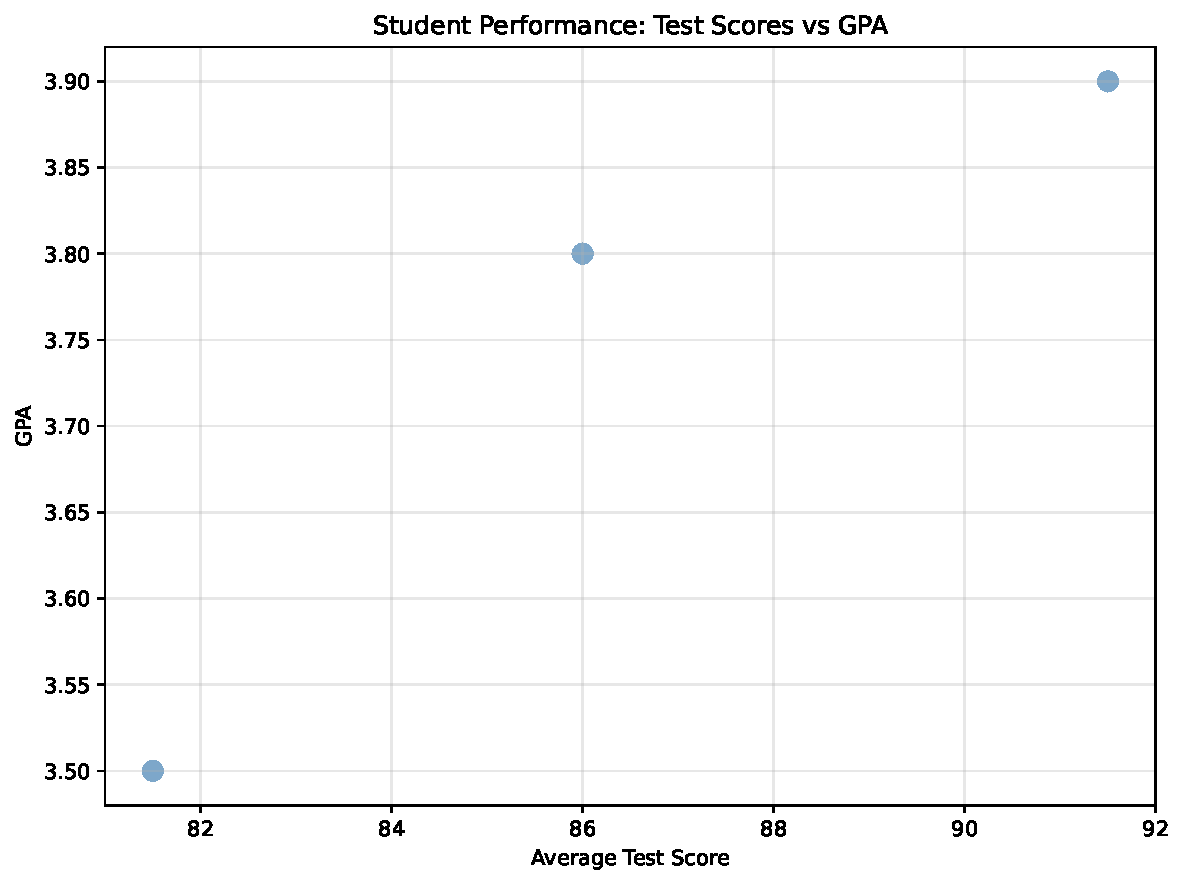
\includegraphics[keepaspectratio]{index_files/figure-pdf/fig-student-performance-output-1.pdf}}

}

\caption{\label{fig-student-performance}Relationship between GPA and
average test scores}

\end{figure}%

\textsubscript{Source:
\href{https://BenJPanackal.github.io/me-as-package/index.qmd.html}{Article
Notebook}}

The visualization in Figure~\ref{fig-student-performance} shows the
strong correlation between academic performance metrics, illustrating
how organized data reveals patterns that raw, messy data obscures.

\footnote{By: Ben Panackal}

\textsubscript{Source:
\href{https://BenJPanackal.github.io/me-as-package/index.qmd.html}{Article
Notebook}}

\protect\phantomsection\label{refs}
\begin{CSLReferences}{1}{1}
\bibitem[\citeproctext]{ref-mckinney2010}
McKinney, Wes. 2010. {``Data Structures for Statistical Computing in
Python.''} \emph{Proceedings of the Python in Science Conference},
56--61. \url{https://pandas.pydata.org/}.

\end{CSLReferences}




\end{document}
